% !TEX TS-program = pdflatex
% !TEX encoding = UTF-8 Unicode
% !TEX root = ../main.tex
% !TEX spellcheck = en-US
% ****************************************************************************************
% File: behaviour.tex
% Author: Jakob Spindler
% Date: 2024-06-01
% ****************************************************************************************
\chapter{Behaviour of the turtle}
\label{chapter:behaviour_of_the_turtle}

The following \autoref{fig:turtlesim_examples_a_to_d} shows examples of the turtle's behaviour, showcasing that the \texttt{turtlesimAutomata} package is working as intended.


\begin{figure}[htbp]
    \centering
    \begin{subfigure}[b]{0.40\textwidth}
        \centering
        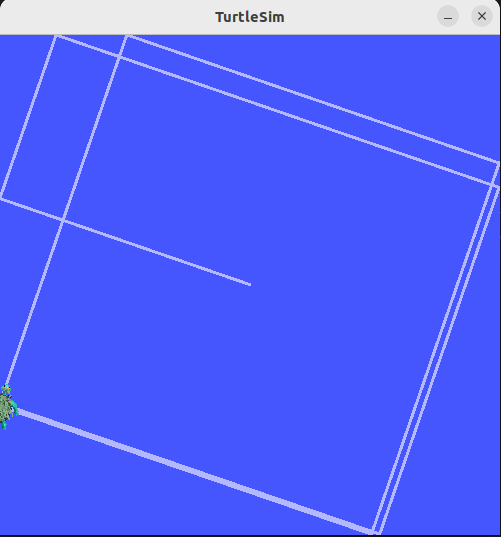
\includegraphics[width=\textwidth]{turtle_example1.png}
        \caption{}
        \label{fig:example_a}
    \end{subfigure}
    \hfill
    \begin{subfigure}[b]{0.40\textwidth}
        \centering
        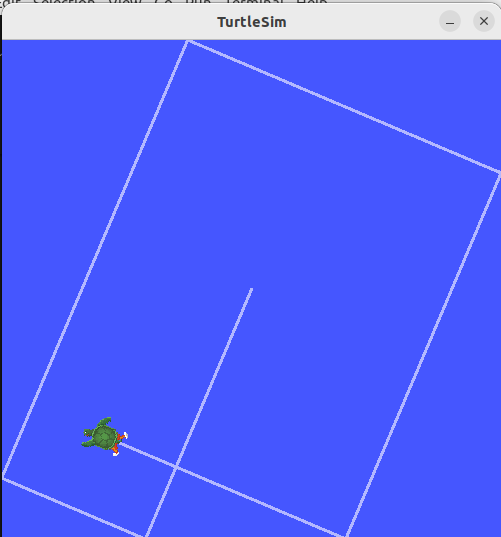
\includegraphics[width=\textwidth]{turtle_example3.png}
        \caption{}
        \label{fig:example_b}
    \end{subfigure}
\\
    \centering
    \begin{subfigure}[b]{0.40\textwidth}
        \centering
        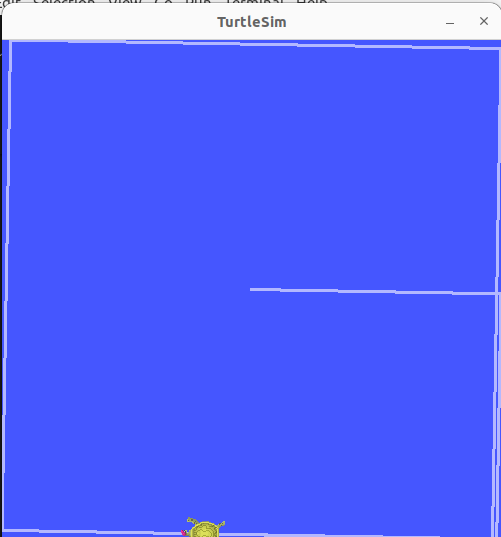
\includegraphics[width=\textwidth]{turtle_example5.png}
        \caption{}
        \label{fig:example_c}
    \end{subfigure}
    \hfill
    \begin{subfigure}[b]{0.40\textwidth}
        \centering
        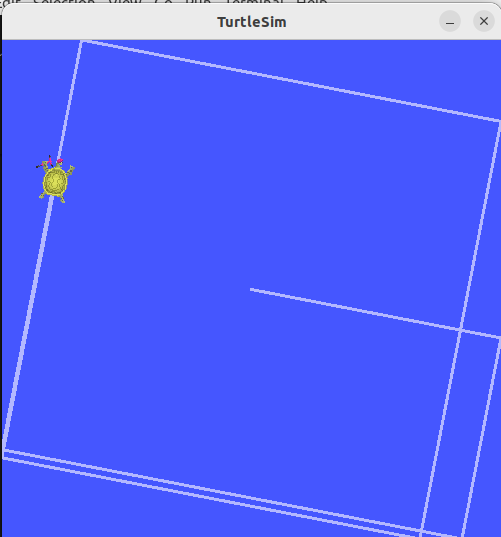
\includegraphics[width=\textwidth]{turtle_example4.png}
        \caption{}
        \label{fig:example_d}
    \end{subfigure}
    \caption{Examples of the turtle's behaviour}
    \label{fig:turtlesim_examples_a_to_d}
\end{figure}


% EOF